\documentclass{../../Latex_Template/Homework/homework}
\usepackage[utf8]{inputenc}
\usepackage{float}

% Graphics Path
\graphicspath{ {images/} }

% CHANGE THE FOLLOW THREE LINES!
\newcommand{\hwname}{Wu, Bo-Run}
\newcommand{\hwstudentid}{r08942073}
\newcommand{\hwnum}{1}
\newcommand{\hwtype}{Homework}
\newcommand{\hwsection}{}
\newcommand{\hwlecture}{}
\newcommand{\hwclass}{FinTech}
\newcommand{\hwdate}{2020-10-24}

\begin{document}

\maketitle

\question*{Linear Regression}
  \begin{alphaparts}
    \questionpart
    For splitting training and testing sets, I use the numpy package to shuffle
    the indexes, by calling \emph{random.permutation} function. Then, I choose
    the first 80\% indexes to be training set, and else to be testing set. Also,
    I use the pandas package to transform the binary columns to one-hot encoding
    vectors by calling \emph{get\_dummies()}, and normalize the data by apply
    normalize function column by column.

    \questionpart
    RMSE: 12.14.

    \questionpart
    RMSE: 11.95. The loss function that add the regularization term is 

    \questionpart
    $\frac{1}{2}||\boldsymbol{X^{(train)}w - Y}||^2_2 + \frac{\lambda}{2}
    \boldsymbol{w^T w}$
    and we let the first derivative of the loss function to be zero. $ 
    \boldsymbol{X^{(train)} (X^{(train)}w - Y)} + \lambda \boldsymbol{w} = 0$
    and we can get the $\boldsymbol{w = (X^{(train)T} X^{(train)} + \lambda
    )^{-1}  X^{(train)T} Y}$ as the closed form solution.

    \questionpart
    RMSE: 3.68.

    \questionpart
    RMSE: 3.68.

    \questionpart
    The figure \ref{fig:student_line_chart} is the predicted G3 values and
    RSMEs for (b) - (e). The reason why (d) and (e) are more closer to the
    Ground Truth is that the $\boldsymbol{w}$ from (d) and (e) are the same
    under the assumption of (e). As we can see in the figure
    \ref{fig:student_line_chart}, (b) with the regularization has the
    improvement that variance between the predicted values get smaller, and the
    (c) with both regularization and bias shift the (b) curves with constants
    letting (c) to be more closer to the Ground Truth. 
    \begin{figure}[h]
      \centering
      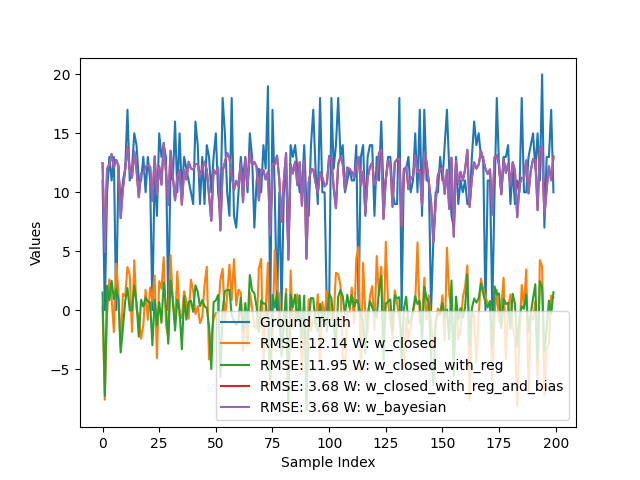
\includegraphics[width=0.5\linewidth]{student_line_chart}
      \caption{Student Line Chart}
      \label{fig:student_line_chart}
    \end{figure}

    \questionpart
    The result is written in the r08942073\_1.txt
  \end{alphaparts}
        

\question*{Census Income Data Set}
As we change the data set to census income data set, the problem become
logistic regression instead of linear regression. The first problem that we
encounter is the missing value in this data set. Fortunately, the missing value
are all in the categorical columns, e.g. the columns without continuous values,
so I specify another label for the columns that have missing value to represent
the missing value. Next, I solve this problem by using linear regression to
minimize the root-mean-square error between the predicted results and the ground
truths. Here, I transform the ground truths into 0 and 1, representing two
different level of income. The solution is not the traditional way of solving
logistic regression, but we can see the differences from Problem 1. As we can
see in the figure \ref{fig:census_bar_chart}, the regularization didn't help
the model to predict, and the bias did.
    
\begin{figure}[h]
  \centering
  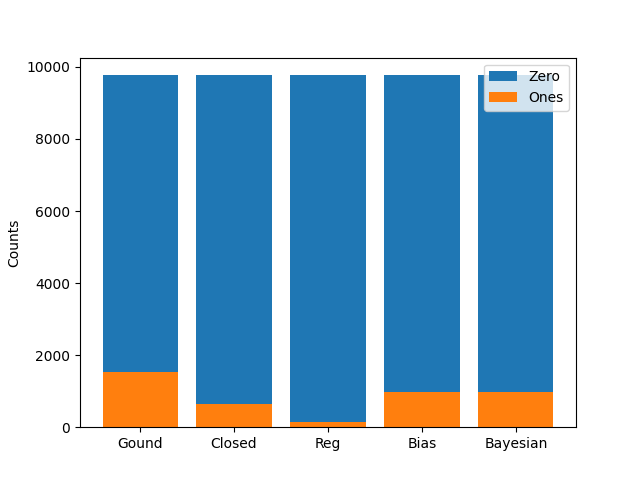
\includegraphics[width=0.5\linewidth]{census_bar_chart}
  \caption{Census Bar Chart}
  \label{fig:census_bar_chart}
\end{figure}


\end{document}
